\chapter{Geheugencel}
\label{cell}
De meeste geheugenschakelingen bestaan uit een verzameling individuele cellen die op een bepaalde manier informatie bevatten.
In dit hoofdstuk wordt dieper ingegaan op de manier waarop een RRAM geheugencel informatie bevat.

\section{Memristor}
Het essentiële element van de RRAM geheugencel is de zogenaamde memristor.
Volgens de originele memristortheorie (zie bijlage \ref{Chua}) is dit de 4\textsuperscript{e} passieve component, naast de weerstand, spoel en condensator. De resistief schakelende elementen die in de praktijk gebruikt worden stroken echter met deze theorie, maar zullen in wat volgt toch memristors genoemd worden.

\subsection{Fysische memristors}
Er werd reeds langer (zelfs al sinds de jaren 60) opgemerkt dat sommige metaaloxides, die normaal gezien als elektrisch isolator functioneren, een plotse overgang kunnen vertonen naar een veel hogere staat van geleiding (zie figuur \ref{fig:i-v}). Dit gebeurt veelal in een configuratie waarbij het oxide wordt geplaatst tussen 2 metalen (MIM configuratie)\cite{Won12} (zie ook figuur \ref{fig:mim}). In die vroege jaren werd er reeds gesuggereerd dat deze structuren gebruikt konden worden voor geheugentoepassingen\cite{Sim67}, maar de elementen bleken niet stabiel genoeg voor circuitimplementatie. Bovendien waren de siliciumgebaseerde geheugens in opmars, waardoor er geen nood was voor verder onderzoek.

\begin{figure}[ht!]
  \centering
  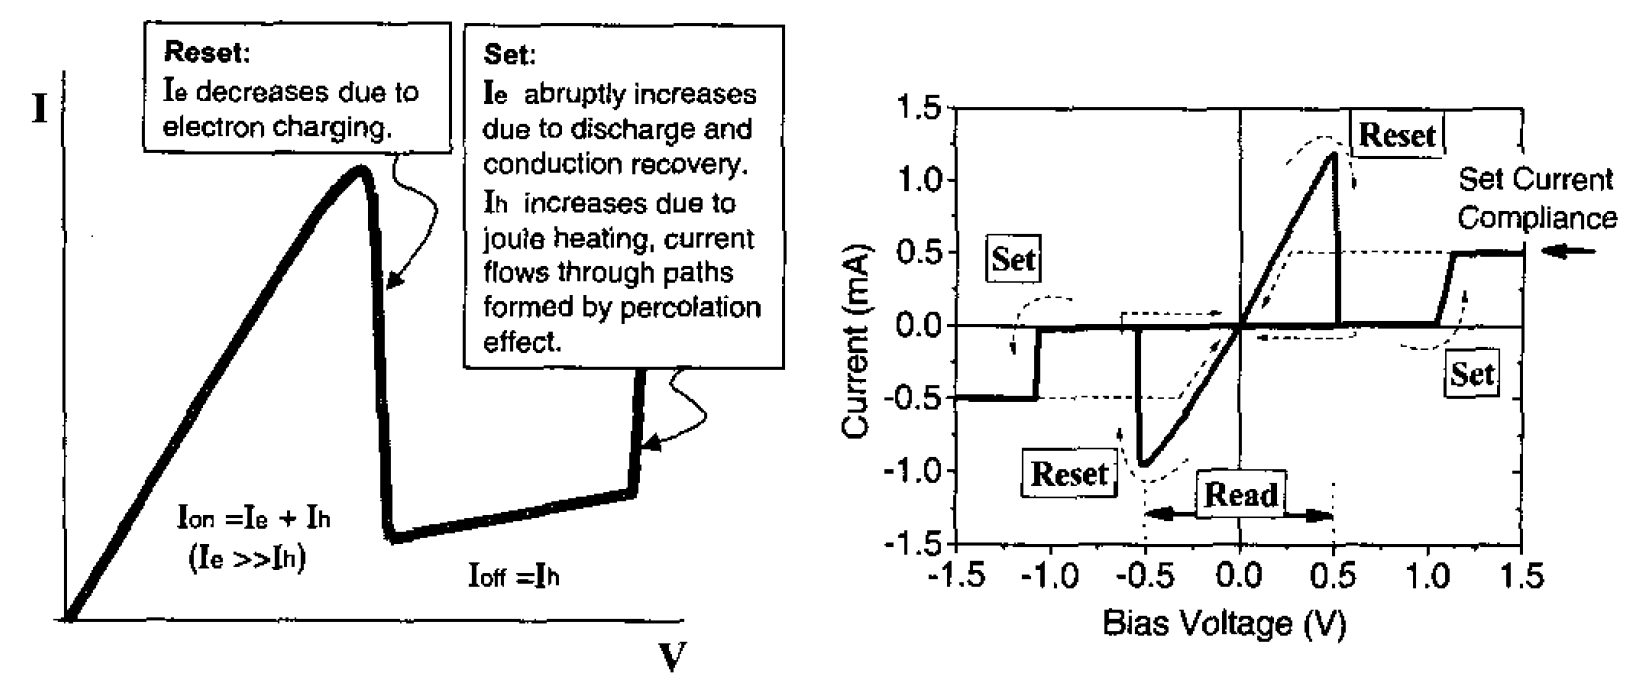
\includegraphics[scale=0.20]{../fig/hfdstk-cel-I-V.png}
  \caption[Resistieve schakeling]{Overgang van hoge weerstand naar lage weerstand voor NiO bij DC analyse (unipolaire memristor), reproduced from\cite{Bae04}}
  \label{fig:i-v}
\end{figure}

\begin{figure}[ht!]
  \centering
  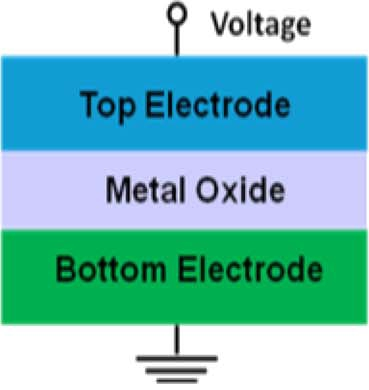
\includegraphics[scale=0.35]{../fig/hfdstk-cel-MIM.png}
  \caption[MIM structuur]{Metal-Insulator-Metal structuur, reproduced from\cite{Won12}}
  \label{fig:mim}
\end{figure}

In het begin van het nieuwe millennium wakkerde de interesse voor resistief schakelende elementen weer aan door enkele nieuwe ondezoekspublicaties zoals \cite{Bec00} en \cite{Zhu02}, waarin veel stabielere resitieve elementen werden gepresenteerd. Zhuang et al. brachten ook de term RRAM aan in hun artikel. In 2008 publiceerde een onderzoeksgroep van Hewlett-Packard een artikel waarin ze opmerkten dat het gedrag van hun Pt-TiO\textsubscript{2}-Pt stalen een merkwaardige gelijkenis vertoonde met Chua's originele memristortheorie\cite{Str08}. Uit de modellering van hun stalen argumenteerden ze dat dit een ideale memristor zou zijn en dat het effect meer uitgesproken is bij kleine afmetingen. Het titaniumoxide bestaat o.w.v. niet-idealiteiten uit 2 delen: zuiver TiO\textsubscript{2}, een halfgeleider met hoge weerstand, en TiO\textsubscript{2-x} met zuurstofafwezigheid (oxygen vacancies) met een veel lagere weerstand. Door een elektrisch veld aan te leggen worden zuurstofatomen weg of in het rooster getrokken en verandert de verhouding TiO\textsubscript{2} en TiO\textsubscript{2-x} en dus ook de netto weerstand (zie figuur \ref{fig:HP-model}).

\begin{figure}
  \centering
  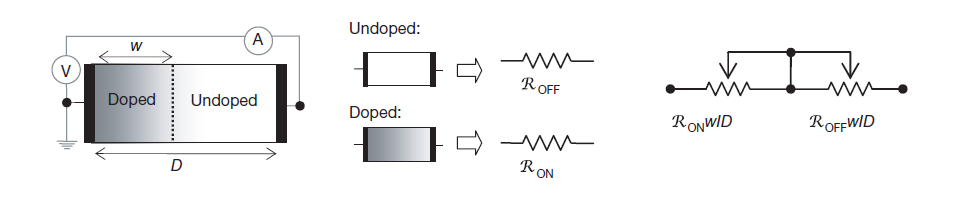
\includegraphics[scale=0.5]{../fig/hfdstk-cel-HP-model.png}
  \caption[Model van het Pt-TiO\textsubscript{2}-Pt staal]{Model van het Pt-TiO\textsubscript{2}-Pt staal, reproduced from\cite{Str08}}
  \label{fig:HP-model}
\end{figure}

Voor deze opstelling geldt dan dat $M(q)=R\textsubscript{off}(1-\frac{\mu\textsubscript{v}R\textsubscript{on}}{D^2}q(t))$ met M de \emph{memristance}, D de totale dikte van de titaniumoxidefilm, $\mu\textsubscript{v}$ de mobiliteit van de zuurstofionen en $R\textsubscript{on} \leq M \leq R\textsubscript{off}$. Het dymamisch gedrag van de ogenblikkelijke weerstandswaarde is dus afhankelijk van het verloop van de stroom in de tijd en dit effect treedt des te meer op in het nanometerdomein.

Er zijn nog talloze andere materialen die schakelend weerstandsverdrag vertonen zoals nikkeloxide\cite{Bae04}, hafniumoxide\cite{Che11}, aluminiumoxide\cite{Kim06},... Niet altijd kunnen de resultaten gemodelleerd worden volgens de originele memristortheorie, maar desalnietemin zullen deze materiaalconfiguraties bruikbaar zijn in toepassingen en zullen ze in de rest van dit werk memristoren genoemd worden.
Bij al deze MIM-configuraties blijft het mechanisme wel hetzelfde: na fabricatie is het oxidekristal intrinsiek zuiver, maar onder druk van een voldoende groot elektrisch veld zullen de zuurstofatomen losgerukt worden uit het rooster naar de anode. Het gebrek aan zuurstofatomen zorgt voor conductieve filamenten. Het element bereikt dan een laagresistieve staat (LRS).
Deze zachte doorslag van het zuivere oxide wordt \emph{forming} genoemd. Het proces is tot zekere hoogte omkeerbaar (\emph{reset}), maar er zullen altijd meer defecten in het kristal zijn dan voor de forming. Dit betekent dus ook dat nadat de memristor één keer een forming- en resetproces is ondergaan en zich terug in een hoogresistieve staat (HRS) bevindt, er hierna een minder groot elektrisch veld nodig is om terug tot een LRS te komen. Dit proces heet \emph{setting}. Deze drie processen zijn geïllustreerd op figuur \ref{fig:forming-reset-set}.

\begin{figure}
  \centering
  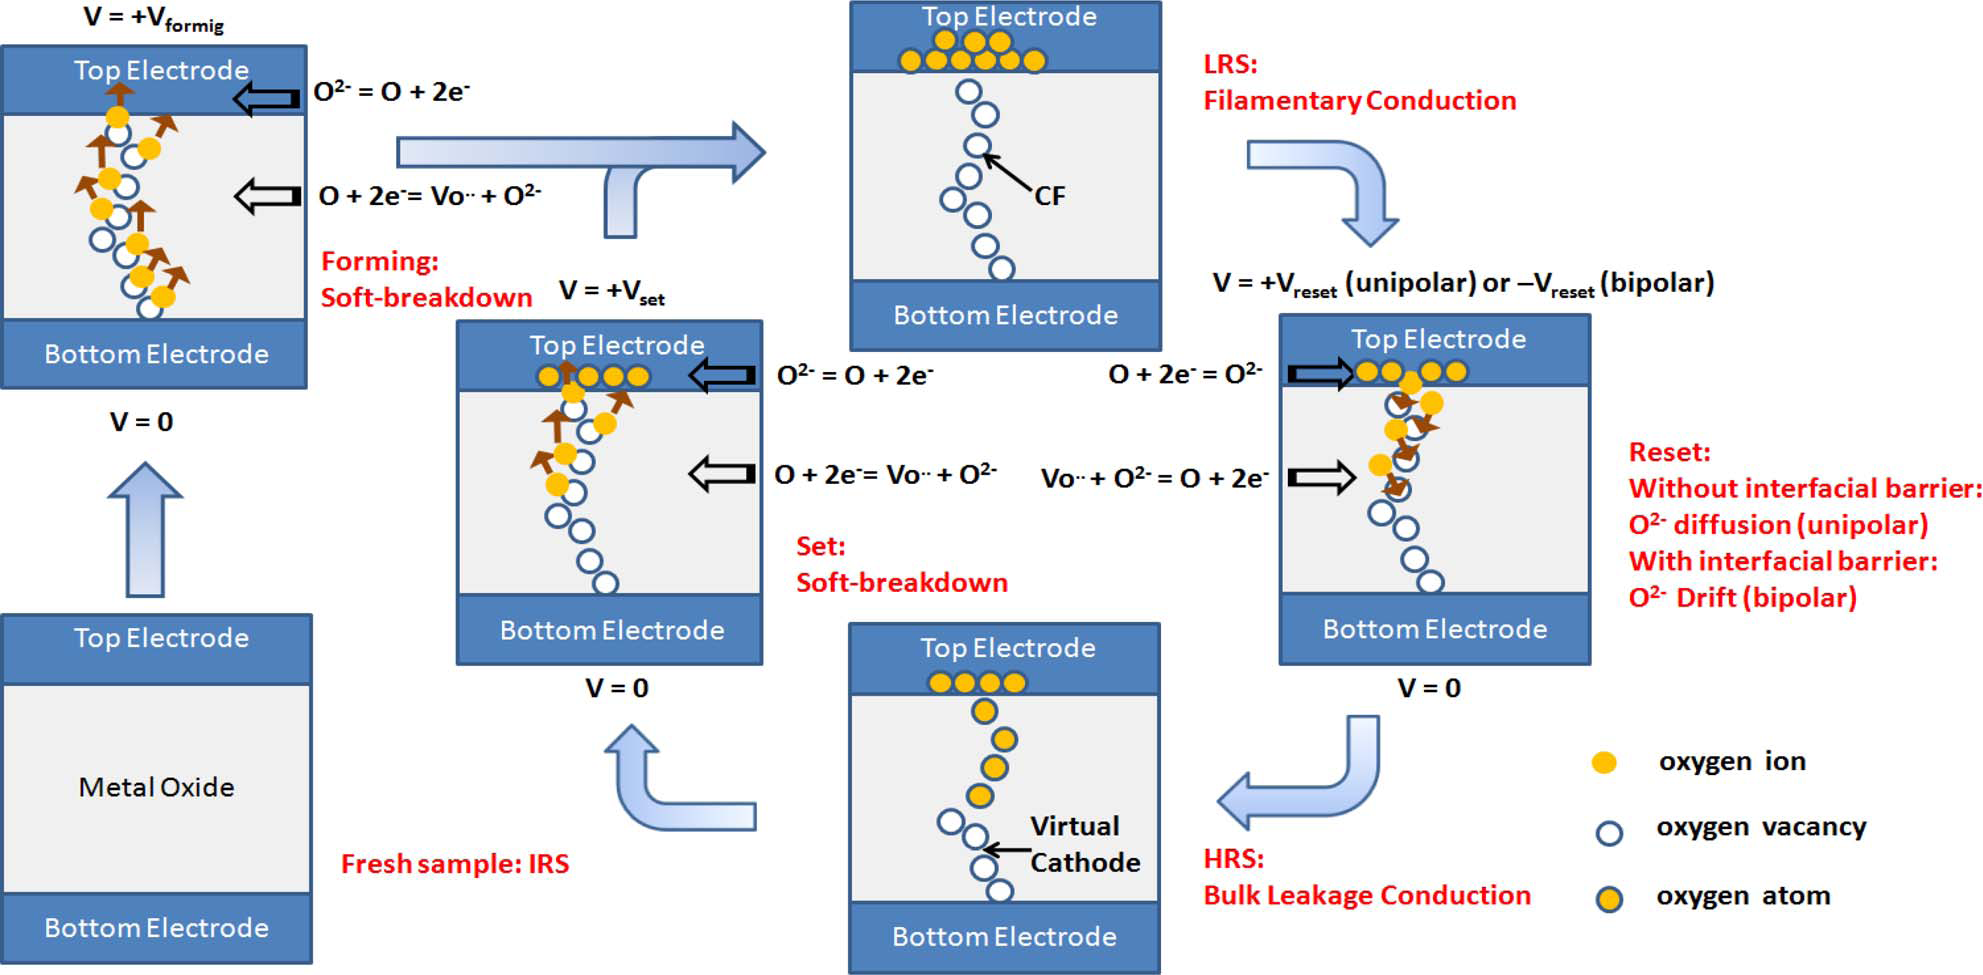
\includegraphics[scale=0.22]{../fig/hfdstk-cel-forming-reset-set.png}
  \caption[Forming,resetting en setting van een memristor]{Illustratie van forming,resetting en setting, reproduced from\cite{Won12}}
  \label{fig:forming-reset-set}
\end{figure}

MIM-structuren gefabriceerd uit verschillende materialen hebben ook verschillende eigenschappen. Zo moet er onderscheid gemaakt worden tussen unipolair schakelen en bipolair. Bij bipolair resistief schakelen zal forming/setting optreden wanneer de aangelegde spanning een bepaalde polariteit heeft en resetting bij de omgekeerde polariteit. Bij unipolair schakelen is de amplitude of de duur van de spanning doorslaggevend voor welke van de 3 processen zal optreden, niet de polariteit. DC-analyses voor biplaire en unipolaire memristors staan afgebeeld op figuur \ref{fig:bipolar-unipolar}.

\begin{figure}
  \centering
  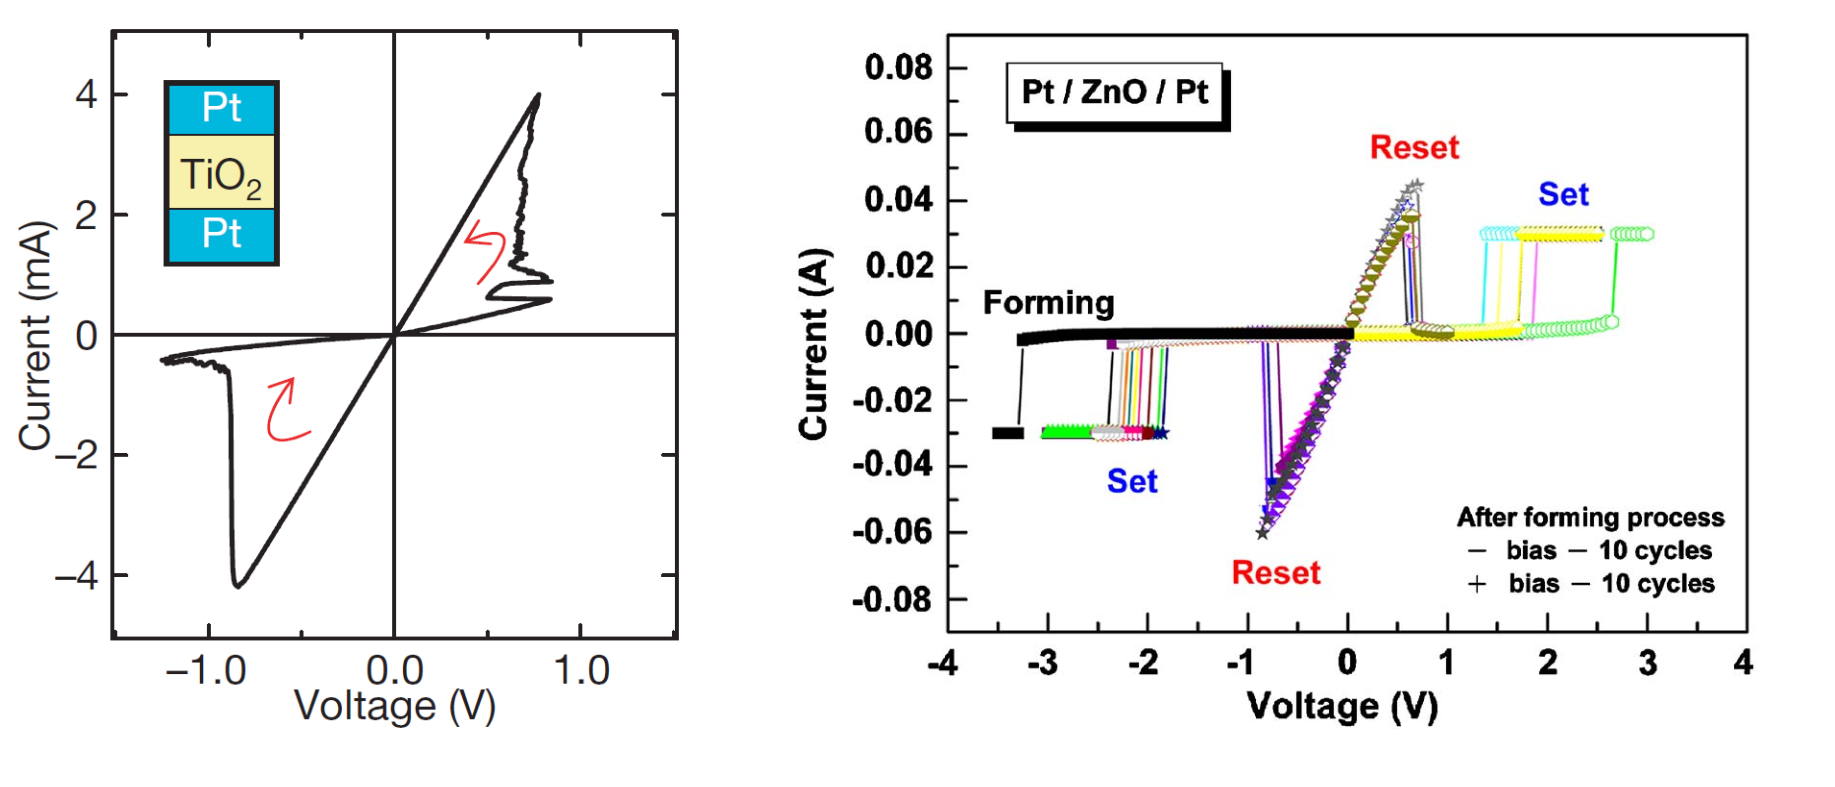
\includegraphics[scale=0.27]{../fig/hfdstk-cel-bipolar-unipolar.png}
  \caption[DC-analyse bipolaire/unipolaire memristor]{DC-analyses bipolaire en unipolaire memrisors, reproduced from \cite{Str08} \& \cite{Cha08}}
  \label{fig:bipolar-unipolar}
\end{figure}


\section{Memristorconfiguraties}

\subsection{Algemene configuraties}
Op basis van deze bevindingen kan de memristor gebruikt worden als geheugenelement: de MIM-configuraties hebben op z'n minst 2 resistieve toestanden, al zijn er artikels gepubliceerd waarbij de memristor nog meer resistieve toestanden bevat\cite{Liu12}. Als deze multiresistive states onder controle gehouden kunnen worden, kan een nog hogere densiteit aan informatie gerealiseerd worden aangezien elke memristor meer dan 1 bit informatie zou bevatten (multi-level cells).
Deze 2 toestanden kunnen gebruikt worden voor geheugen- en logicatoepassingen\cite{ros12}\cite{raj09}. In geheugentoepassingen kan men onderscheid maken tussen 1T1R-,1R- en 1D1R-configuraties\cite{Den13}. Met een 1R-configuratie kan men de grootste densiteit van geheugen bereiken, alsook een betere schaling, maar deze configuratie heeft te kampen met cellen die half geselecteerd worden en lekstroom. Dit kan opgelost worden door een selectie-element aan de configuratie toe te voegen, zoals een diode of een transistor. De 1D1R configuratie kan echter enkel geïmplementeerd worden met unipolaire memristors\cite{Wou09}. Daarom is er in dit werk voor een 1T1R-configuratie geopteerd. De memristor waarop dit werk gebaseerd is, is immers een bipolaire hafniumoxide-memristor (zie figuur \ref{fig:1T1R}).

\begin{figure}
  \centering
  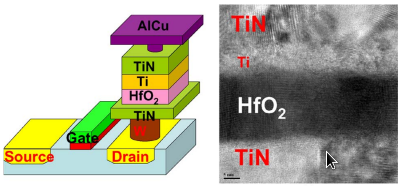
\includegraphics[scale=0.6]{../fig/hfdstk-cel-1T1R.png}
  \caption[Een 1T1R-configuratie]{Een 1T1R-configuratie, reproduced from\cite{Won12}}
  \label{fig:1T1R}
\end{figure}

Naast geheugentoepassingen heeft de memristor ook potentieel in logicatoepassigen en er wordt zelfs gesproken over een mogelijke vervanger van de transistor\cite{Kue05}.
\subsection{1R-cel}
\label{1R}
The 1R-configuratie bestaat uit 1 memristor. Deze cel kan dan verbonden worden aan een WL en BL. Deze structuur die beter bekend is als een \textit{crossbar array} kan een geheugenmatrix vormen met een heel hoge densiteit. Een van de problemen waarmee deze configuratie te kampen heeft bij de leesoperatie is echter het \textit{read sneak leakage path}\cite{leakpath}(figuur \ref{fig:leak}). Bij de leesoperatie wordt er een spanningsdeling uitgevoerd tussen de memristor en een lastimpedantie. Bij een \textit{crossbar array} gaan er echter lekstromen gevormd worden die door andere cellen vloeien. Dit zorgt voor een parallelle weerstand die heel afhankelijk is van de resistieve staat van de cellen in de geheugenmatrix. Volgens \cite{5763125} kan dit probleem opgelost worden door de resterende WL te biasen of door de leescyclus in twee stappen uit te voeren. Bij deze laatste oplossing gaat men eerst de lekstroom van het circuit opmeten en deze vervolgens aftrekken van de totale leesstroom.

\begin{figure}
  \centering
  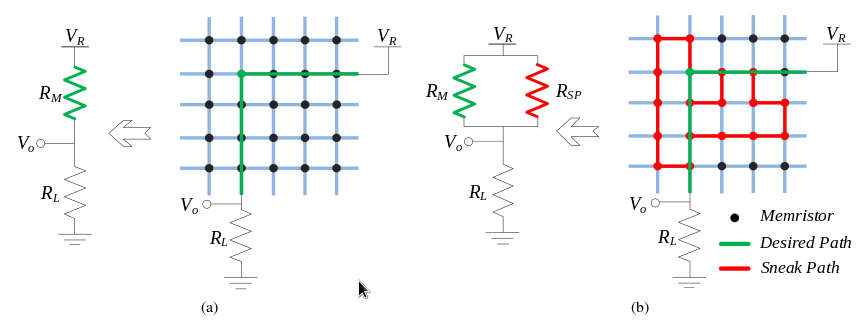
\includegraphics[width=\textwidth]{../fig/hfdstk-cel-1Rleak.png}
  \caption[Read sneak leakage path]{Read sneak leakage path, reproduced from\cite{leakpath}}
  \label{fig:leak}
\end{figure}

De schrijfoperatie heeft dan weer te kampen met een probleem dat het \textit{write half-select problem} heet (figuur \ref{fig:halfselct}). Hierbij gaan cellen die op dezelfde BL of WL liggen als de geselecteerde cel, half geselecteerd zijn. De uitdaging hierbij is om te garanderen dat deze cellen niet van resistieve staat veranderen. Er bestaan verschillende biasing methodes \cite{1269425} om dit probleem te overkomen. Bij het schrijven van meerderen cellen tegelijkertijd, kunnen methodes zoals \textit{SET-before-RESET} of \textit{ERASE-before-RESET}\cite{5763125} gebruikt worden.

\begin{figure}
  \centering
  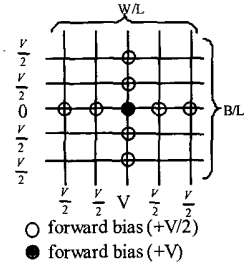
\includegraphics[width=0.5\textwidth]{../fig/hfdstk-cel-halfselect.png}
  \caption[Half select problem]{Half select probleem, zwarte cellen zijn volledig geselecteerd, witte cellen zijn half geselecteed, reproduced from\cite{1269425}}
  \label{fig:halfselct}
\end{figure}

\subsection{1T1R-cel}
\label{1T1R}
De 1T1R-configuratie bestaat uit 1 CMOS-transistor en 1 memristor in serie geschakeld. De cel kan  worden verbonden in een matrix zoals geillustreerd in figuur \ref{fig:1T1R-schematic}. Een woordlijn wordt verbonden aan de gate van de transistor, de source van de transistor wordt verbonden aan een sourcelijn en tenslotte wordt een bitlijn gehangen aan de vrije terminal van de memristor. Ook lees- en schrijfoperaties worden geïllustreerd op figuur \ref{fig:1T1R-schematic}. De leesoperatie is in wezen een spanningsdeling tussen de impedantie van de cel en een andere lastimpedantie die de BL verbindt met de voedingsspanning. Om een logische 1 te schrijven kan de BL rechtstreeks worden aangesloten aan de voedingsspanning. De stroom door de memristor is hierbij groter dan bij leesoperatie en de memristor (indien die zich nog niet in de gewenste resistieve staat bevond) gaat schakelen naar de gewenste resistieve staat. Om een logische 0 te schrijven staat er op de BL de grondspanning en op de SL de voedingsspanning. De stroom vloeit nu in de omgekeerde richting.

\begin{figure}[!ht]
\centering
\subfloat[Algemeen schema]{ 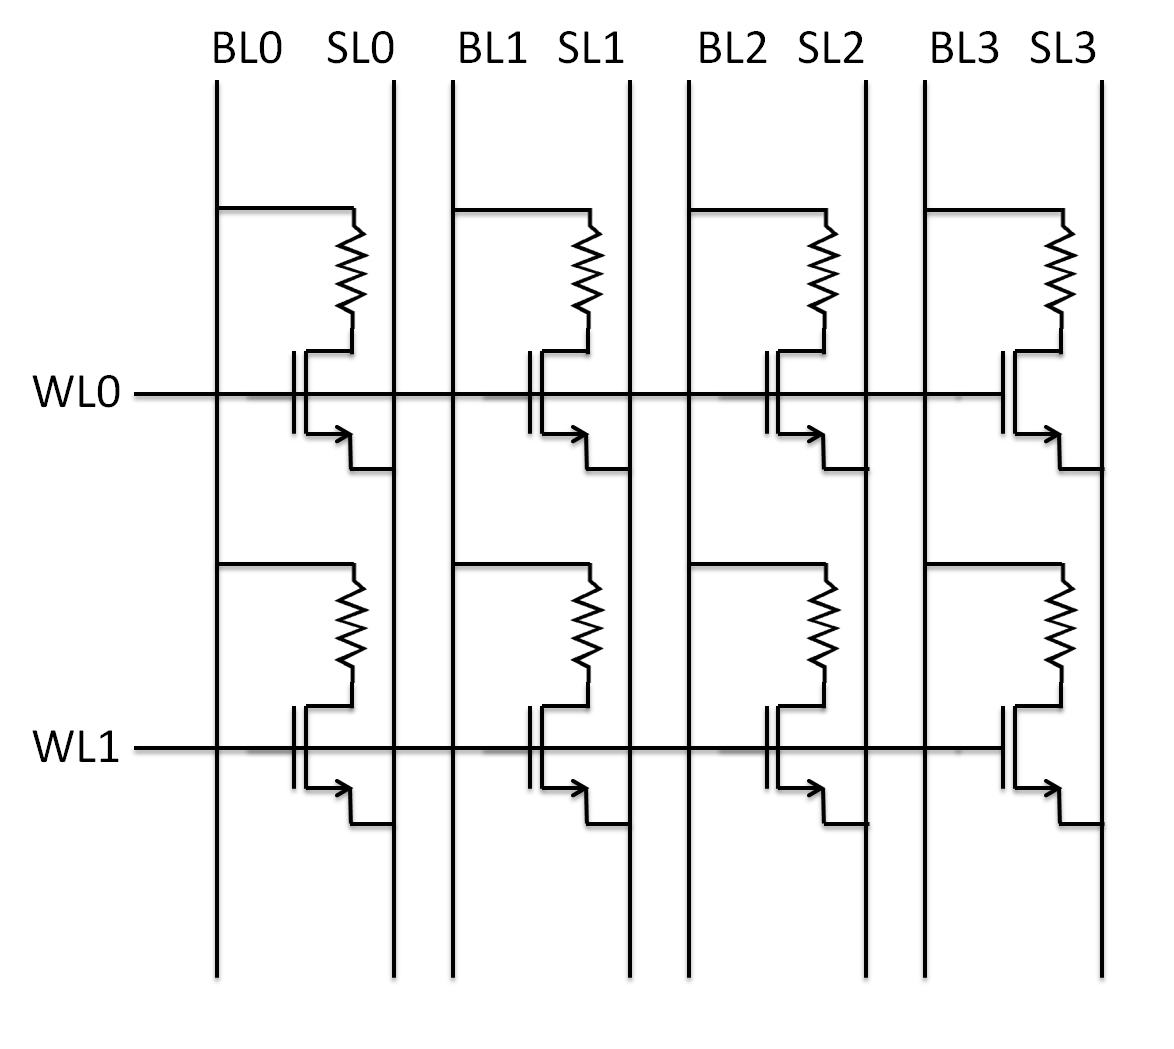
\includegraphics[width=0.5\textwidth] {../fig/hfdstk-cel-1T1R-schematic.png}}
\subfloat[Leesoperatie]{ 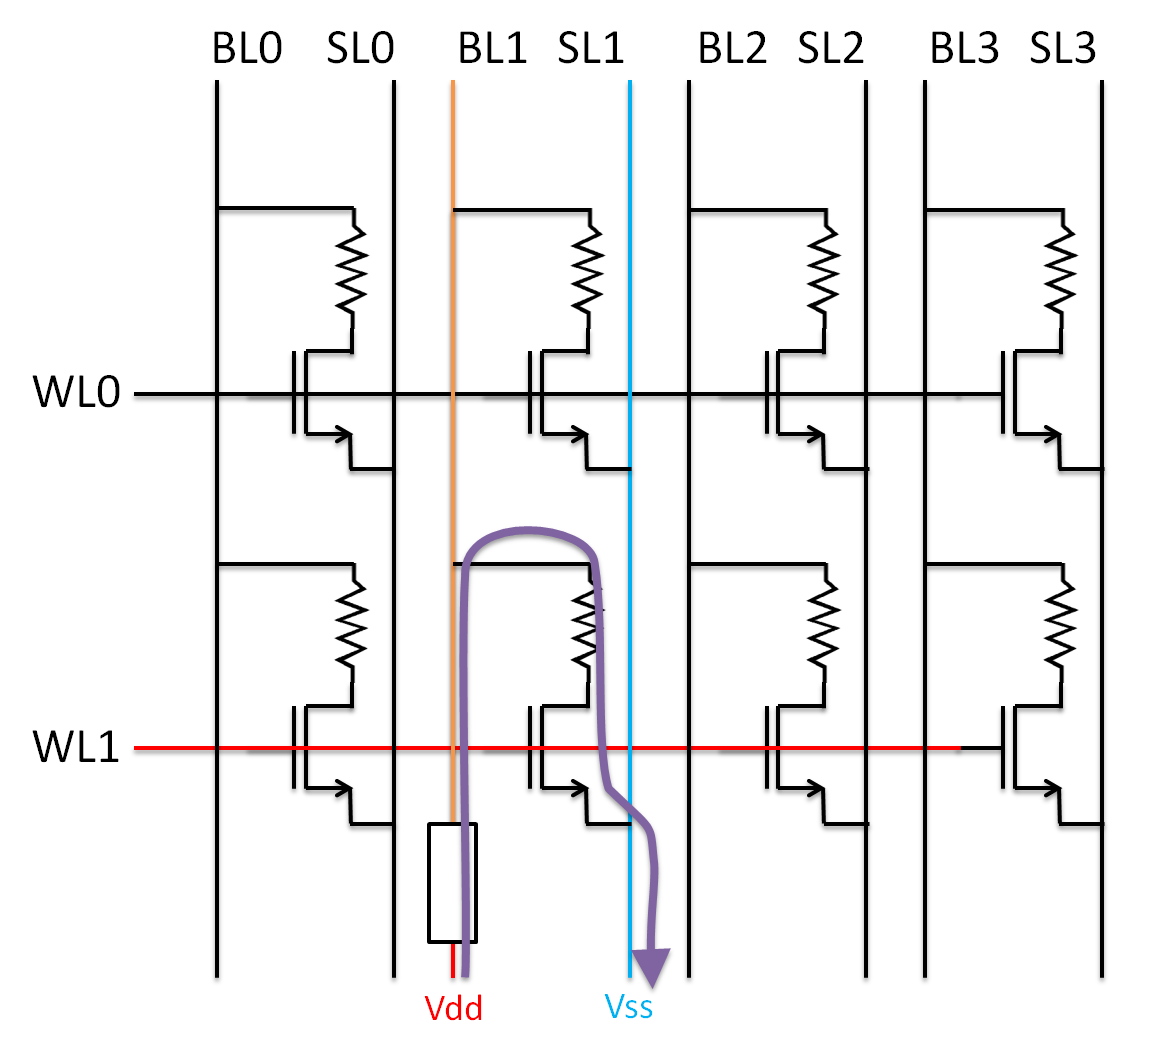
\includegraphics[width=0.5\textwidth] {../fig/hfdstk-cel-1T1R-read.png}}\\
\subfloat[Schrijfoperatie voor een 1]{ 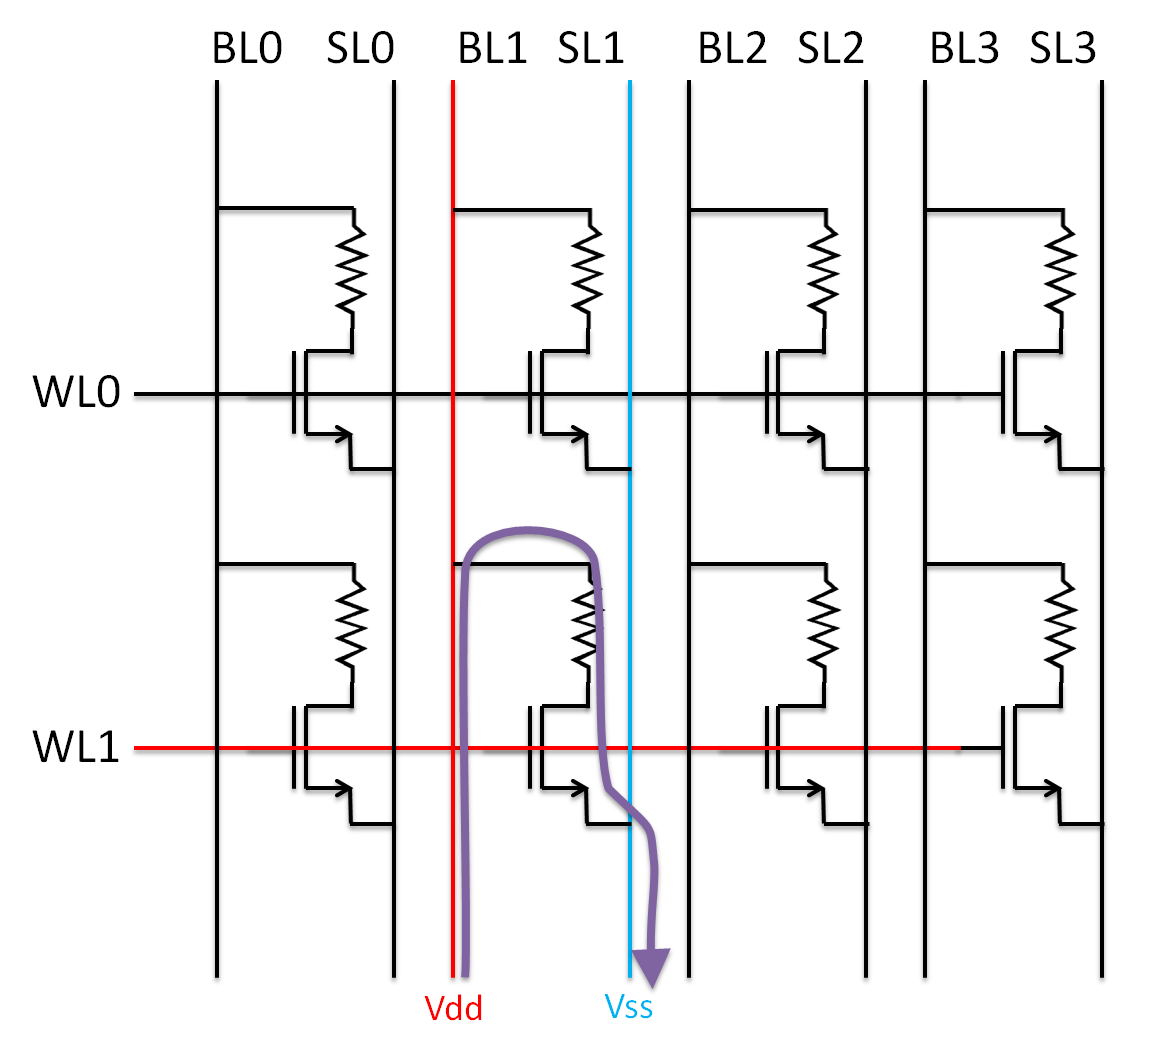
\includegraphics[width=0.5\textwidth] {../fig/hfdstk-cel-1T1R-write1.png}}
\subfloat[Schrijfoperatie voor een 0]{ 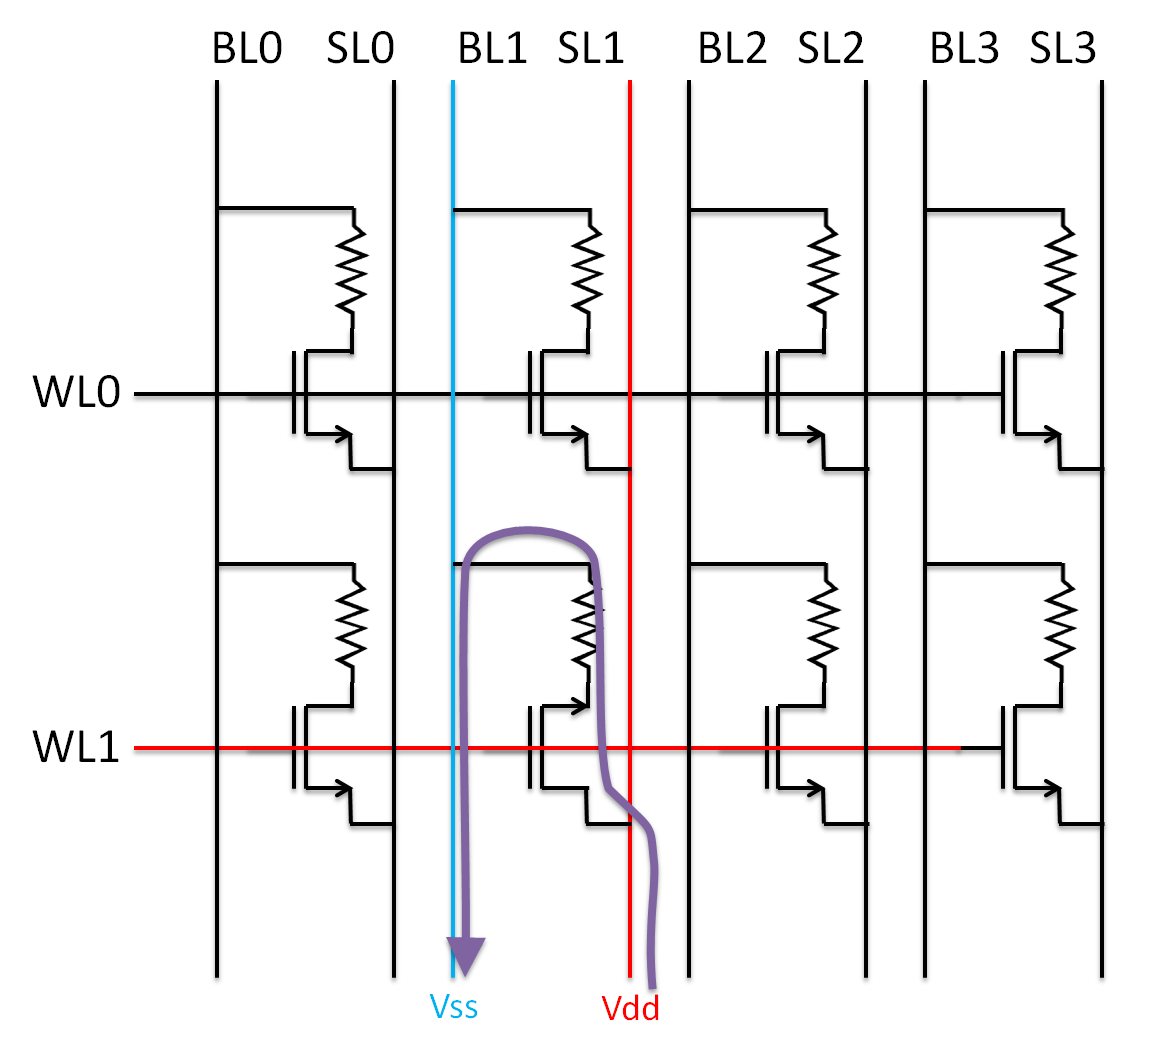
\includegraphics[width=0.5\textwidth] {../fig/hfdstk-cel-1T1R-write0.png}}\\
\caption[1T1R matrix]{1T1R matrix met verschillende operaties}
\label{fig:1T1R-schematic}
\end{figure}

\section{Besluit}
De memristor is een theoretische passieve component die kan gemodelleerd worden via een verband tussen lading en elektrische flux. In de praktijk zijn er MIM-configuraties ontdekt die (gedeeltelijk) memristorkarakteristieken vertonen. Deze karakteristieken zijn bijzonder interessant voor geheugens: gecombineerd met een transistor vormt de memristor een 1T1R-geheugencel, die geïmplementeerd wordt in de volgende hoofdstukken.
